\subsection{Stress tests and extreme sparsity}
\label{sec:synthetic}
\begin{figure}[t]
\centering
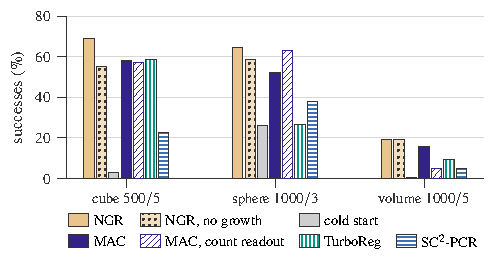
\includegraphics[width=\columnwidth]{figures/fig_sparse.pdf}
\caption{Frozen synthetic benchmark (250 inputs per setting, $N/m$: matches/inliers). Inliers are noisy transformed points, and outliers are uniform in the unit cube (cube), in a radius-5 ball (sphere) or in the object's bounding box (volume). Success: RE $<5^\circ$, TE $<0.05$. The same NGR seeds are fitted directly or grown. MAC is the authors' C++ code with its compatibility width fixed to 0.75$\tau$ (\supp{\cref*{S-sec:s-maccpp}}); hatched bars show it with NGR's count readout. On the volume background, NGR uses MAE and MAC keeps its own choice. Full protocols and fresh draws are in Supp.~Sec.~\ref*{S-sec:s-synthetic}.}
\label{fig:sparse}
\end{figure}

\Cref{tab:units}a isolates seeded growth on the dilute volume inputs: pair nuclei improve from 2/40 without growth to 19/40 with ten stages. Resetting half the composition each stage removes most of the pair-seeded gain, supporting retained enrichment.

On the frozen cube setting in \cref{fig:sparse}, removing growth lowers NGR from 69.2\% to 55.2\%. With three sphere-background inliers among 4000 matches, NGR registers 29/100 inputs versus at most 4/100 for SC$^2$-PCR and TurboReg. On real scans thinned to 5 to 20 inliers no frontend consistently leads. Full grids and tests are reported in \supp{\cref*{S-sec:s-synthetic}}.
